\documentclass{article}

% Language setting
% Replace `english' with e.g. `spanish' to change the document language
\usepackage[english]{babel}

% Set page size and margins
% Replace `letterpaper' with`a4paper' for UK/EU standard size
\usepackage[a4paper, total={7in, 9in}]{geometry}

% Useful packages
\usepackage{amsmath}
\usepackage{graphicx}
\usepackage[colorlinks=true, allcolors=blue]{hyperref}

\title{\textbf{Domain-aware Aligner Documentation}}
\author{\textbf{Group 5}}

\begin{document}
\maketitle

\section{Major task}

This software developed an algorithm to align protein sequences considering their domain composition. Modular proteins can undergo domain loss or acquisition because of long genomic insertions, deletions, and duplications. Current alignment algorithms maximize an alignment score based on a match/mismatch and gap score. The domain content of a protein can be predicted with tools like \href{http://pfam.xfam.org/}{Pfam} or \href{https://www.ebi.ac.uk/interpro/}{InterPro}, and the predictions are already available in databases such as \href{https://www.uniprot.org/}{Uniprot}. \textbf{Proteins with various domain architectures frequently produce poor results when aligned using current, reliable tools}. With the use of pairwise alignments and an algorithm that considers domain architectures, this software aims to produce all multiple sequence alignments.

\section{Input and Output}
\begin{enumerate}
\item The \textbf{input section} includes the original sequences data (\textbf{fasta, txt}…) and annotated \textbf{tsv} data for target protein families from the Uniprot database (annotation data is an \textbf{optional input}). You can also use the built-in simulate data of this algorithm.
\item The \textbf{output section} includes the following four parts:
\begin{itemize}
\item \textbf{Fasta} result from Domain-wise Greedy MSA
\item \textbf{Fasta} result from HMM-based Domain-level Alignment
\item Running logs of the algorithm (including unmatched information, and will be put on the screen)
\item Sum-of-pairs score of the alignment result (\textbf{optional})
\end{itemize}
\end{enumerate}\\

\begin{figure}
\centering
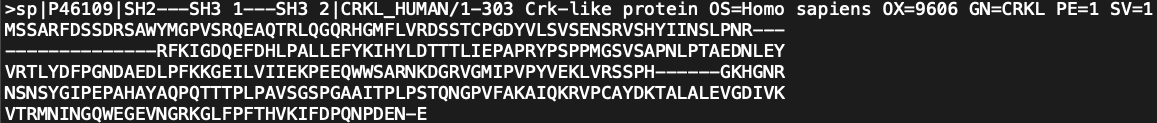
\includegraphics[scale=0.45]{1.png}
\caption{\label{fig:1}CRK's category wise results.}
\end{figure}

\section{Key algorithms}
Our core algorithm can be divided into two modules: domain-wise greedy MSA and HMM-based domain-level alignment. Domain-wise greedy MSA module categorizes protein sequences according to their domain composition (categorize\_seqs\_by\_domain\_info), and then use a progressive greedy algorithm to perform MSA on each of the domains and linkers in the sequences for each category. Specifically, hierarchical clustering was performed on all sequences based on hamming distance between their pairwise alignments (calculate\_pairwise\_distance\_matrix). Then, MSA was generated gradually by merging sequence clusters based on the clustering result (merge\_two\_sequence\_clusters). Pairwise alignments are implemented using a dynamic programming approach with three score and backtrack matrices to represent three affine gaps and match states (affine\_gap\_penalties\_pair\_wise\_alignment). Then domain-level information was then used to build a customized Hidden Markov Model (HMM) to profile domain arrangement pattern (construct\_HMM). A special state, 'SWAP' was added to this model, to represent the situation that two domains exchanging their position to map sequence (align\_to\_SWAP\_HMM). We implement the Viterbi learning algorithm to iteratively train our model (HMM\_Viterbi\_Learning). After the model has been well trained, we perform HMM-based align for each input sequence (merge\_hidden\_paths) and merge then to a uniform pattern for further operation including benchmarking. For further implementation details including IO and helper functions, please refer to our source code.

\section{Setting up running environment}
\begin{itemize}
\item This program requires python 3.7 or above. Please first ensure the python environment of the device
\item The input sequences should be biological data of queriable modular proteins with \textbf{at least 2 domains} with \textbf{Uniprot Entry ID} (for compatibility with HMM model) downloadable from UniProt database. We also support testing on an internally simulated data set. 
\item Make sure that all python dependency packages have been correctly installed (shown in Installation)
\end{itemize}

\section{Installation}
There are three prerequisites that users need to satisfy:
\begin{enumerate}
\item Downloaded the compressed file of the software (\textbf{zip file})
\item Input: annotated information provided by the \href{https://www.uniprot.org/}{Uniprot} database (\textbf{optional}, not necessary in networking conditions)\\
the \textbf{tsv} file should contain at least two columns of \textbf{Entry} and \textbf{Domain [FT]}
\item Installed the \textbf{python modules} required by the software algorithm:
\begin{itemize}
\item \textbf{numpy 1.23.5}
\item \textbf{blosum 1.2.2}
\item \textbf{argparse 1.4.0}
\item \textbf{pandas 1.5.2}
\item \textbf{bs4 0.0.1}
\end{itemize}
\end{enumerate}

\noindent Use \textbf{pip} to install the required modules:\\
\textbf{\$ pip install numpy blosum argparse pandas bs4}

\section{Parameters and Explanation}
\begin{itemize}
\item \textbf{-h}  \textbf{(Optional)} it will return a explanation of the parameters usage
\item \textbf{-i}  \textbf{(Optional)} the path to read in raw sequences file, or \textbf{ignore this parameter to use the build-in simulated data}
\item \textbf{-o}  \textbf{(Required)} the path to save the result fasta file, default path is current system path
\item \textbf{-ref\_mode}  \textbf{(Required)} ref\_mode must be in one of \textbf{['tsv', 'uniprot', 'simulate']}, \textbf{database reference selection}, 'simulate' means to use the build-in simulate data
\item \textbf{-r}  If ref\_mode is in \textbf{‘tsv’}, r must be the path to read in uniprot reference tsv file
\item \textbf{-sigma}  \textbf{(Optional)} set the gap open penalty, enter an \textbf{integer}, default value is 11
\item \textbf{-epsilon}  \textbf{(Optional)} set the gap extension penalty, enter an \textbf{integer}, default value is 1
\end{itemize}

\section{Test running instruction}

You can follow the following reference steps to run the program:
\begin{itemize}
\item A zip file of the program is available from our \href{https://github.com/Yifei-Shang42/BMI3_domain_aware_aligner/blob/main/BMI3_domain_aware_aligner.zip}{GitHub}
\item Download the zip file of the program to a local directory, and use the \textbf{\$ unzip} command on the terminal to extract the program
\item Use the \textbf{\$ cd} command to change the current path to the program folder
\item Run the code using the following usage template:
\begin{enumerate}
\item \$ python main.py \textbf{-i} SRC.fasta \textbf{-o} \textbf{-ref\_mode} uniprot \textbf{-sigma} 10
\item \$ python main.py  \textbf{-o} \textbf{-ref\_mode} simulate
\item \$ python main.py \textbf{-i} CRK.txt \textbf{-o} \textbf{-ref\_mode} tsv \textbf{-r} /crk\_uniprot.tsv
\item \$ python eval.py \textbf{-i} result\_HMM.fasta
\end{enumerate}
\end{itemize}

\section{Readme file}

This software is based on \textbf{python3.7 or later}. For data alignment, this algorithm will \textbf{occupy a large memory}. Therefore, please use it properly based on your operating device. Before using this software, {ensure that you have installed python packages} such as \textbf{numpy 1.23.5, blosum 1.2.2, argparse 1.4.0, pandas 1.5.2, and bs4 0.0.1} in your python environment.
This software zip file contains five python script files, as well as three test cases.\\

\noindent The input sequences should be biological data of queriable modular proteins with \textbf{at least 2 domains} with \textbf{Uniprot Entry ID} (for compatibility with HMM model) downloaded from UniProt database. We also support testing on an internally simulated data set.\\

\noindent What you could to operate are the \textbf{main.py and eval.py}.\\
\noindent \textbf{main.py} will produce the domain-wise greedy MSA alignment, the alignment sequence result of HMM-based Domain-level alignment and the visualization figure.\\
\noindent \textbf{eval.py} will calculate the sum-of-pairs score of the alignment.\\

\noindent \textbf{Usage of this software:}\\
\$ python main.py \textbf{-i} [input file path] [\textbf{-o} output file path] \textbf{-ref\_mode} ['tsv', 'uniprot', 'simulate'] [\textbf{-r} uniprot tsv file path] [\textbf{-sigma} int] [\textbf{-epsilon} int]\\
\$ python eval.py \textbf{-i} [input file path]\\

\noindent \textbf{Example1:}\\
\$ python main.py \textbf{-i} SRC.fasta \textbf{-o} \textbf{-ref\_mode} uniprot \textbf{-sigma} 10\\
\noindent \textbf{Example2:}\\
\$ python main.py  \textbf{-o} \textbf{-ref\_mode} simulate \\
\noindent \textbf{Example3:}\\
\$ python main.py \textbf{-i} CRK.txt \textbf{-o} \textbf{-ref\_mode} tsv \textbf{-r} /crk\_uniprot.tsv\\
\noindent \textbf{Example3:}\\
\$ python eval.py \textbf{-i} result\_HMM.fasta\\

\noindent \textbf{Developers:}\\
Biomedical Informatics 3 mini-project Group5

\end{document}
